%!TEX root = main.tex

\section{Die Thurston-Norm}
	
	Nun wollen wir zu der ersten der beteiligten Normen kommen --- der Thurston-Norm. Um den roten Faden und die Motivation zu bewahren sei der Beweis von Theorem~\ref{thm:haupttheorem} wiefolgt skizziert: Zunächst soll $b_1(\ker\phi)=b_1(M_\phi)$ als untere Schranke für die Auswertung der Thurston-Norm an dem surjektiven $\phi \in H^1(M;\ZZ) = \Hom (\pi_1(M);\ZZ)$ herausgestellt werden. Dann wird die Auswertung der Alexander-Norm an einem surjektiven $\phi$ in Zusammenhang mit $b_1(\ker\phi)$ gesetzt. Die Kombination dieser Ergebnisse wird das Theorem liefern. Dieses Kapitel widmet sich der Definition der Thurston-Norm und der unteren Abschätzung durch $b_1(\ker\phi)$.

	\subsection{Eigenschaften der Thurston-Norm}

        Wir haben in Kapitel~\ref{sec:poinc} und \ref{sec:constr} gesehen, wie jede Homologieklasse in $H_2(M,\partial M;\ZZ)$ (ggf.\,$\partial M=\emptyset$) dual zu $\phi \in H^1(M;\ZZ)$, durch eine glatte Einbettung einer orientierten Fläche repräsentiert ist. Dies  ermöglicht die Definition der Thurston-Norm:
        \begin{defn}[Thurston-Norm]
        	Definiere die Thurston Norm für $\phi \in H^1(M,\ZZ)$ als
        	\[
        	        		||\phi||_T = \min\{ \chi_-(S)| ~(S,\partial S) \subset (M,\partial M)\text{ ist orientierte eingebettete Fläche dual zu } \phi \},
        	        	\]        	
        	wobei $\chi_-(S)=\sum \max (-\chi(S_i),0)$ und über $S=\sqcup S_i$ die Zusammenhangskomponenten von $S$ summiert wird.
        \end{defn}
        
        Das folgende Ergebnis ist von Thurston~\cite{Thurston.1986}.
        \begin{lem}
        \label{lem:norm}
        	Die Thurston Norm definiert eine Halbnorm auf $H^1(M;\ZZ)$ und somit auf $H^1(M;\RR)$. 
        \end{lem}
          \noindent\textit{Beweis.}
          Die Fortsetzung auf $H^1(M;\RR)$ wurde in Lemma~\ref{lem:fortsetzungnorm} behandelt.

          Es muss die Skalarmultiplikativität und die Subadditivität gezeigt werden, also:
            \begin{align}
                ||\lambda\phi||_T & = \lambda ||\phi||_T ,&\lambda \in\ZZ \label{eq:scalarmul} \\
                ||\phi + \psi||_T &\leq ||\phi||_T + ||\psi||_T ,& \phi,\psi \in H^1(M) \label{eq:subadd}
            \end{align} 

            Da die Thurston Norm aus den Eigenschaften der dualen Flächen hervorgeht, ist es nötig sich Gedanken zu den dualen Homologieklassen zu machen. Dann ist es für \eqref{eq:scalarmul} offensichtlich hinreichend, falls für repräsentierende, orientierte, eigentlich eingebettete Flächen, etwa $S,T$ mit Bildern ihrer Fundamentalklassen $[S],[T]\in H_2(M,\partial M)$ und $[S]=\lambda [T]$, die Fläche $S$ bereits disjunkte Vereinigung von $\lambda$ Komponenten $S_i$ ist, mit $[S_i]=[T]$. 

			Für $[S]=\phi \in H^1(M;\ZZ)$ existiert eine glatte Abbildung $f:M \to S^1$, die $\phi$ repräsentiert und ohne Einschränkung einen regulären Wert $s\in S^1$ habe, dessen Urbild $S$ ist (siehe Kapitel~\ref{sec:poinc} und Konstruktion~\ref{constr:cut} bzw.\,Corollar~\ref{cor:preimage}). Sei auch $g:M \to S^1$ glatt mit dem regulären Wert $t$, sodass $g^{-1}(t)=T$ mit korrekter Orientierung gilt, also $H_1(g)$ dual zu $[T]$ ist. Es gilt $\im\pi_1(f) \subset \lambda \ZZ$, da die induzierte Abbildung der Fundamentalgruppen mit der dualen Kohomologieklasse identifiziert werden kann (vgl.\,Bemerkung~\ref{bem:fundhomologie}), die aber deswegen auch ein $\lambda$-Vielfaches ist. Betrachtet man die Überlagerung $p: S^1 \stackrel {z^\lambda} \to  S^1$, liefert die Überlagerungstheorie einen Lift $\hat f$:
            \[
                \begin{xy}
                    \xymatrix{M \ar[r]^{\hat f} \ar[d]_g \ar[dr]^f&S^1 \ar[d]^p \\
                             S^1 \ar[r]_p & S^1}
                \end{xy}
            \]
            Das Quadrat kommutiert bis auf Homotopie, also $p\hat f \simeq p g$, denn beide Abbildungen identifizieren sich unter der Bijektion $H^1(M;\ZZ) \cong [M,S^1]$ (siehe Kapitel~\ref{sec:poinc}) mit dem Dual von $ \lambda [T]$ etwa $\lambda \phi$, also impliziert die Existenz dieser Bijektion, dass $[p\hat f] = [pg]$. Somit folgt auch (mit Kapitel~\ref{sec:poinc}), dass Urbilder regulärer Werte aus $S^1$ unter $\hat f$ homolog zu solchen aus $g$ sind. Da $p^{-1}(s)=\{s_1,\cdots,s_n\}$ sicherlich reguläre Werte von $\hat f$ sind (folgt zum Beispiel aus der Kettenregel für Differentiale), sind die Urbilder $S_1,\cdots,S_n$ disjunkte, eingebettete, orientierte Flächen mit $[S_i]=[T]$. Da $S$ auch minimal (bezüglich der Thurston-Norm) gewählt werden kann, folgt also $||\lambda \phi||_T \geq \lambda ||\phi||_T $. Nun lassen sich aber aus einer minimierenden Fläche für $[T]$ (sei $T$ ohne Einschränkung selbst so gewählt), zum Beispiel mithilfe eines zweiseitigen Kragens $T \times (-\epsilon,\epsilon) \to M$, $\lambda$ disjunkt eingebettete Kopien von $T$ gewinnen, die offensichtlich auch $[S]$ repräsentieren, also $||\lambda \phi||_T = \lambda ||\phi||_T$. 

            Um nun die Subbadditivität \eqref{eq:subadd} zu zeigen, ist es nötig die Geometrie der $||\cdot||_T$-minimierenden orientierten eingebetteten Flächen $S,T$, mit $[S]$ dual zu $\phi$ und $[T]$ dual zu $\psi$, genauer zu betrachten. Die Differentialtopologie liefert mit dem Transversalitätstheorem (vergleich Kapitel~\ref{sec:poinc}) diffeotope (also insbesondere homologe) Approximationen von $T$, die transversal zu $S$ sind, deswegen seien also ohne Einschränkung $S \transversal T$ transversal. Außerdem folgt durch die Transversalität, dass $S\cap T$ eine glatte, kompakte 1-Mannigfaltigkeit ist, man sagt auch "`Der Pullback der Einbettungen bleibt in der Kategorie"'. Die Klassifikation von kompakten 1-Mannigfaltigkeiten liefert, dass dieser Durschnitt eine disjunkte Vereinigung von Kreisen und kompakten Intervallen ist (letztere existieren natürlich nur, wenn $S,T$ und somit $M$ Rand haben). Des Weiteren existiere ohne Einschränkung der Allgemeinheit keine Kreiskomponente des Schnittes $S\cap T$ die eine Scheibe berandet, die in $S$ oder $T$ enthalten ist. Diese Annahme kann man wie folgt rechtfertigen:

                        \begin{wrapfigure}{r}{0.55\textwidth}
                \centering
                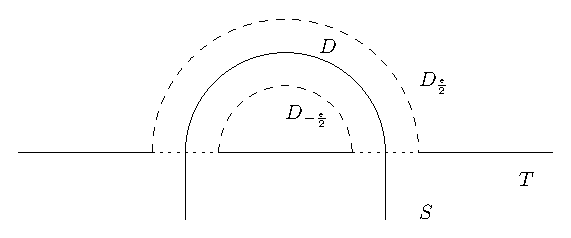
\includegraphics[width=0.54\textwidth]{surgery}
                \caption{Ausschneiden einer Umgebung von $S\cap T$ und Ankleben zweier Scheiben, sodass die Homologieklasse erhalten bleibt}
                \label{fig:surgery}
            \end{wrapfigure} 
            Angenommen es existiert ein Nullbordismus $D\subset S$ einer Komponente $\partial D \subset S \cap T$. Weiter sei dieser auf dem Inneren disjunkt von $T$, da ein nichttrivialer Schnitt mit $T$ einen weiteren Kreis aus $S\cap T$ liefert, der den Nullbordismus einschränkt, sodass er weniger Komponenten im Schnitt mit $T$ berührt als der ursprüngliche (man bemerke das Transversalität genutzt wurde). So fahre man endlich oft fort, bis der Durchschnitt mit $T$ trivial ist, also die berandende Scheibe in $S$ die Fläche $T$ nur im Rand berührt.
            Nun lässt sich eine offene Tubenumgebung von $\partial D \subset T$ aus $T$ entfernen.
			Diese kann wie folgt gewählt werden: Sei $\nu(S) \to M$ eine Tubenumgebung von $S$, die sich aufgrund der Zweiseitigkeit wie folgt wählen lässt: $\alpha: S \times (-\epsilon,\epsilon) \to M$, sodass $\im\alpha|_{S\times (-\frac 12\epsilon,\frac 12 \epsilon)} \cap T$ eine Tubenumgebung von $S\cap T $ in $ T$ ist. Dann lässt sich diese Tubenumgebung an $\partial D$ aus $T$ entfernen und mittels des betrachteten zweiseitigen Kragens von $S$ um $D$ findet man zwei Kopien $D_{\frac \epsilon 2}, D_{-\frac \epsilon 2}$, sowie Anklebevorschriften, mit denen diese Scheiben an die beiden durch Ausschneiden entstandenden Kreis-Randkomponenten von $T$ kleben kann, vergleiche Abbildung~\ref{fig:surgery}. Da die Tubenumgebung (die Flächen sind kompakt) so gewählt werden kann, dass für jedes $|\delta|<\epsilon$ die glatte Einbettung $\alpha|_{S \times \{\delta\}}$ transversal zu $T$ ist, liefert die Tubenumgebung Informationen zum Glätten der entstehenden Untermannigfaltigkeit $T'$ \footnote{vgl.\,\cite{WhiteheadJ.H.C..1961} oder man verwende glatte Approximation der topologischen Einbettung mit Wahl einer glatten Struktur der topologischen Mannigfaltigkeit $T'$, vgl.\,\cite[Chapter 5, Lemma 1.5]{Hirsch.1991} und dass $DIFF=TOP=PL$ gilt für Mannigfaltigkeiten in Dimensionen $\le 3$, da dort die Hauptvermutung gilt, vgl.\,\cite[Chapter 35,36]{Moise.1977}} \todo{not sure about this}. Als Resultat ergeben sich die orientierten, glatten Flächen $S \pitchfork T'$, deren Durchschnitt um eine Komponente reduziert wurde und offensichtlich $[T]=[T']$ gilt. Mit einem ähnlichen Argument schließt man kompakte Intervalle $(I,\partial I) \to (S\cap T, \partial(S\cap T))$ aus, die relativ Randpunkten diffeotop zu einer Randkomponente sind. 

            Von nun an seien $S$ und $T$ transversale Flächen, deren Durchschnitt den obigen Anforderungen genügt. Ziel ist es nun den Zykel $[S]+[T]$, als eingebettete Fläche zu repräsentieren. Durch $S$ und $T$ ist bereits ein Repräsentant als Immersion der disjunkten Vereinigung gegeben, da die Fundamentalklasse der disjunkten Vereinigung aus den Fundamentalklassen der Komponenten besteht. Beachtet man die Orientierungen, so kann man an jeder Komponente des Durchschnitts $S\cap T$ die Vereinigung $S\cup T$ aufschneiden (die lokal aussieht wie die Gerade, an der sich zwei orientierte Ebenen im $\RR^3$ schneiden), und entlang der Orientierungen in nur einer Möglichkeit wieder verkleben, so dass man eine Mannigfaltigkeit erhält (dies funktioniert offensichtlich an den Durchschnittkomponenten mit Rand, aber auch an den geschlossenen Komponenten, da die Orientierungen auf $S$ und $T$ global gewählt sind). Natürlich können mit entsprechenden Umgebungen, alle diese Klebe- und Schneideprozesse wieder glatt durchgeführt werden. Nun erhält man eine glatte, orientierte Fläche $U$, die (nach gegebenfalls leichter Modifikation) auch eigentlich eingebettet ist. Für den Wert von $[U]$ unter der Thurston-Norm, muss dieses Ergebnis und die Auswirkungen der Konstruktionen auf die Flächen diskutiert werden. Die obigen "`uneinschränkenden"' Konstruktionen zu Beginn können natürlich die Euler Charakteristik $\chi$ verändern, nicht jedoch $\chi_-$, also resultieren daraus weiterhin Thurston-Norm minimierende Flächen\footnote{Dies geschieht zum Beipsiel durch die Entstehung von Sphären, siehe Abbildung~\ref{fig:surgery}. Wichtig ist nur, dass solche Komponenten nicht beim Verkleben der beiden Flächen entstehen. Genau deswegen wurde diese Annahme getroffen.}. Zwei {solche} Flächen gegeben, erbt die letztere Konstruktion, die aus $S\cup T$ eine homologe Fläche $U$ macht, die Summe der Eulercharakteristika. Dies Vererbung resultiert zum Beispiel aus der Vererbung der CW-Struktur von $U$ aus gegebenen CW-Strukturen von $S$ und $T$ die jeweils $S\cap T$ in ihrem 1-Skelett enthalten. Eine solche Verfeinerung der CW-Strukturen auf $S$ und $T$ lässt sich offensichtlich aus jeder CW-Struktur leicht erreichen. Die folgende Implikation ist im Allgemeinen \emph{nicht} wahr und gilt hier aufgrund der Annahmen an $S$ und $T$, da unter diesen Annahmen bei der Konstruktion von $U$ keine Komponenten mit positiver Eulercharakteristik entstehen.
            \begin{eqnarray*}
                \chi(U) = \chi(S) + \chi(T) &\implies& \chi_-(U)=\chi_-(S) + \chi_-(T)
            \end{eqnarray*}
            Dies liefert nun die Subbadditivität der Thurston-Norm auf den Homologieklassen.
        \qed
        \vspace{6pt}

        Häufig stellt man Annahmen an die 3-Mannigfaltikeit, die es verbieten, dass Homologieklassen von Sphären oder Tori repräsentiert werden können. In dem Fall würde dann sogar $||\phi||_T=0 \Leftrightarrow \phi=0$ gelten. Dies alles motiviert natürlich, diese Norm zu einer Vektorraumnorm auf $H^1(M;\RR)$ fortzusetzen und Lemma~\ref{lem:fortsetzungnorm} belohnt uns mit einer solchen Fortsetzung. 
     
	\subsection{$\thur \cdot$-minimierende Flächen}

Nun wollen wir uns eine besondere Art von Flächen anschauen, nämlich die Repräsentanten der zu $\phi$ dualen Klasse, bei denen $\chi_-$ minimal ist. Dass immer ein Repräsentat existiert, der gewissen Eigenschaften genügt, sichert der folgende Satz:

\begin{lem}
	\label{lem:minS}
	Sei $\phi \in H^1(M;\ZZ)= \Hom (\pi_1(M),\ZZ)$ ein primitives Element und es gelte $b_1(\ker\phi)<\infty$. Dann existiert eine zu $\phi$ duale zusammenhängende Thurston-Norm-minimierende Fläche $(S,\partial S) \subset (M,\partial M)$ mit $b_2(S)=b_3(M)$, so dass folgende Abschätzung erfüllt ist:
	\[
	b_1(S) \leq b_1(\ker(\phi))
	\]
\end{lem}
\begin{proof}
	Wähle unter allen Thurston-Norm-minimierenden Flächen eine orientierte Fläche $S$ mit einer geringsten Anzahl an Zusammenhangskomponenten.\\
	\textit{Behauptung: Diese Fläche ist zusammenhängend}.
	Man betrachte den aus $S$ entstehenden Graphen nach Konstruktion~\ref{constr:graph}.
	Wir werden zeigen, dass unter der Minimalitätsanforderung von $S$ unter diesen Identifikationen klar ist, dass $G$ ein topologischer Kreis ist und $G\to S^1$ die Identität. Das impliziert die Behauptung.

	Dafür betrachte man folgendes Diagramm von Pullbacks von Überlagerungen:

	\[
	 	\begin{xy}
	 		\xymatrixcolsep{4pc}\xymatrix{
	 			M_\phi \ar[r] \ar[d] & G_\phi \ar[d] \ar@{-->}@/_/[l]_{\alpha_\phi} \ar[r] & \RR \ar[d]\\
	 			M \ar[r] & G \ar@{-->}@/_/[l]_\alpha \ar[r] &S^1
	 		}
	 	\end{xy}
	 \] 
	 Man erhält unendlich zyklische Überlagerungen, also unendlich zyklische Decktransformationsgruppen. Unter der oben gezeigten Kompatibilitätsvorraussetzung dieser Überlagerungen durch Pullbacks, mit den Überlagerungen durch Aufschneiden an dualen Flächen (deswegen die suggestive Schreibweise $M_\phi$), entsteht $G_\phi$ durch "`Aufschneiden an den Kantenmitten"'. Nun existieren offensichtlich Homotopieschnitte $\alpha, \alpha_\phi$, also stetige Abbildungen, sodass $ G \stackrel \alpha \to M \to G$ und $ G_\phi \stackrel {\alpha_ \phi} \to M_\phi \to G_\phi$ jeweils homotop zur Identität sind \todo{vgl abbildung}. Mit Funktorialität und Homotopieinvarianz des Homologiefunktors, induzieren $\alpha,\alpha_\phi$ Monomorphismen $H_1(\alpha;\QQ),H_1(\alpha_\phi;\QQ)$, entsprechend sind die ersten Bettizahlen von von $G$ und $G_\phi$ nach oben durch die von $M$ und $M_\phi$ beschränkt. Folglich muss $b_1(G)=1$ sein, sonst wäre $b_1(G_\phi)=\infty> b_1(M_\phi)$, da Fundamentalgruppen von Graphen frei sind. Somit ist $\pi_1(G)= \ZZ$. Also ist $G$ als Graph homotopieäquivalent zu einem Kreis. Da $G$ die Kompaktheit von $M$ erbt, ist nur noch die Existenz von Knoten ohne ein- oder ausgehende Kanten auszuschließen, um zu zeigen das $G$ ein topologischer Kreis ist. Diese ist aber durch die Minimalitätseigenschaft im Bezug auf die Komponenten der gewählten Fläche ausgeschlossen, da solche Kanten einem nullhomologen Zykel entsprechen. Dies sieht man, falls $M$ geschlossen ist, wie folgt ein: Gehöre $M_i$ zu einem ein Knoten der nur eingehende oder nur ausgehende Kanten besitzt, mit den dazugehörigen orientierten Flächen $S_i, i \in I$. Entweder ist dann $(\overline{M_i},\sqcup_{i\in I}S_i)$ oder $(\overline{M_i},-\sqcup_{i\in I}S_i)$ eine Mannigfaltigkeit mit Rand, wobei $-S_i$ die Fläche $S_i$ mit umgekehrter Orientierung bezeichnet, also gilt für das Bild der Fundamentalklasse unter der Inklusion $[-S_i]=-[S_i]$. Ohne Einschränkung gelte der erste Fall. Doch die Inklusion von $\hat S = \sqcup_{i \in I} S$ faktorisiert 
	 \[
	  \hat S \stackrel i \into M = \hat S \stackrel j \into \overline{M_i} \stackrel k \into M,	 	
	 \]
	 und mit der Funktorialität der Homologie faktorisiert auch $H_2(i)=H_2(k)H_2(j)$, aber die Inklusion des Ranges ist homolog trivial $H_2(j)=0$. Hier benutzt man, dass der Rand einer orientierten Mannigfaltigkeit als Homologieklasse mit Kodimension $1$ nullhomolog ist (aus der langen exakten Sequenz für das (orientierte) Paar folgt, dass die Inklusion von Rändern auf der Homologie der Kodimension 1 eine triviale Abbildung induziert, da der Randoperator einen Isomorphismus induziert, der die relative Fundamentalklasse auf die Fundamentalklasse des Randes abbildet). Falls $M$ jedoch nicht geschlossen ist, so folgt mit einem einfachen Schnittzahlenargument, dass jede Homologieklasse als transversale Schleife ausgewertet auf $[\hat S]$ (als duale Kohomologieklasse), die Summe der transversalen Schnitte mit Vorzeichen ergibt, somit $\hat S$ dual zu dem trivialen Homomorphismus $\pi_1(M) \stackrel 0\to \ZZ$ ist, also selbst nullhomolog. Folglich würde dies eine Fläche mit $|I|$ weniger Komponenten und somit einen Widerspruch liefern:
	 \[
	 	[S]=[\sqcup_{i\not \in I} S_i\bigsqcup \sqcup_{i\in I} S_i] = [\sqcup_{i\not \in I} S_i ]+[ \sqcup_{i\in I} S_i] = [\sqcup_{i\not \in I}S_i]
	 \]
	 Betrachtet man nun, wissend dass $G$ ein topologischer Kreis ist, die induzierte Abbildung auf der Homologie $(G\to S^1)_*$, so ist diese ein Isomorphismus, da $\phi$ primitiv ist. Also besitzt $G$ nur eine Kante und die Fläche $S$ ist zusammenhängend.

	 Die nächste Gleichheit --- \emph{die Übereinstimmung des Ranges auf den Top-Homologien von $S$ und $M$} --- hängt von der Existenz eines Randes ab. Da $(S,\partial S) \subset (M,\partial M)$ folgt aus $\partial S \neq \emptyset$ direkt $b_2(S)=b_3(M)=0$. Falls $S$ aber leeren Rand hat, gilt $b_2(S)=1$ und es muss $b_3(M)=1$ gezeigt werden. Dazu wird die Existenz eines Randes von $M$ widerlegt:

	 Nach Annahme existeren nur Tori als Randkomponenten. Sei $T \subset \partial M$ eine solche Randkomponente. Da $S$ keinen Rand hat, also $T$ nicht berührt, enthält die durch Aufschneiden an $S$ erhaltene unendlich zyklische Überlagerung $M_\phi$ auch unendlich zyklisch viele Kopien von $T$ als Randkomponenten. Genauer: Unter Verwendung dieser Aufschneide-Konstruktion~\ref{constr:cut}, liftet $T$ in jedes $M_i \cong M - S \supset T$, auf der sich die Projektion zu einem Diffeomorphismus einschränkt. Im Folgenden soll die Notation $\overline M_i$ für die (wieder) kompakte (Unter-)Mannigfaltigkeit von $M_\phi$ verwendet werden, die den Fundamentalbereich darstellt, der $M_i$ enthält. Zusammen mit der langen exakten Sequenz für eine kompakte orienierbare Mannigfaltigkeit $(N,\partial N)$
	\[
	 \begin{xy}
	 	\xymatrix{
	 	H_2(N;\QQ) \ar[r]&  H_2(N,\partial N ; \QQ) \ar[r]^\delta & H_1(\partial N;\QQ) \ar[r]^{i_*}& H_1(N;\QQ) \\
	 	& &H^1(N;\QQ) \ar[ru]_{\cong} \ar[lu]^{\text{Lefschetz Dualität: }\cong \qquad~}&}
	 \end{xy}
	 \] 
	 und der daraus folgenden Abschätzung
	 \[
	 	b_1(\partial N) = \dim(\im \delta) + \dim(\im i_*) \leq  2b_1(N)
	 \]
	 erhält man für jede kompakte zusammenhängende (man bemerke die implizite Anforderung an $I\subset \ZZ$) Untermannigfaltigkeit der Form 
	 \[
	  	\bigcup_{i\in I} \overline M_i \subset M_\phi 
	  \]
	  die Abschätzung:
	  \[
	   	b_1(\bigcup_{i\in I} \overline M_i)\geq \frac{1}{2}b_1(\partial \bigcup_{i\in I} \overline M_i) \geq \frac{1}{2}b_1(\sqcup_{i \in I}T) = |I|
	  \]


	 \noindent Nun folgt aber aus der Mayer Vietoris Sequenz (für entsprechende offene Umgebungen\footnote{Stichworte hier: das allgemeine Theorem über Tubenumgebungen, Umgebungsdeformationsretrakt}) die exakte Sequenz:
	  \[
	  	\cdots\to H_1(S\sqcup S;\QQ) \to H_1(\bigcup_{i \in I} \overline M_i;\QQ) \oplus H_1(M_\phi -\bigcup_{i \in I} \overline M_i;\QQ) \to H_1(M_\phi;\QQ) \to 0
	  \]
	  und somit
	  \[
	  	b_1(M_\phi)= b_1(\bigcup_{i \in I} \overline M_i)+b_1(M_\phi -\bigcup_{i \in I} \overline M_i)-b_1(S\sqcup S) \geq |I| -2b_1(S)
	  \]
	  Da aber $b_1(M_\phi)$ nach Voraussetzung endlich ist und $|I|$ beliebig groß, folgt also, dass der Rand von $M_\phi$ keine Tori enthält und somit leer ist.

	  Um nun noch\emph{ die Abschätzung $b_1(M_\phi) \leq b_1(S)$ }zu zeigen, wird erneut die Konstruktion der Überlagerung durch Aufschneiden und Verkleben zur Hilfe genommen. Da $\ker\phi \tensor \QQ \cong H_1(M_\phi;\QQ)$ nach Voraussetzung ein endlich erzeugter $\QQ$-Vektorraum ist, wird $H_1(M_\phi;\QQ)$ von einem kompakten Teilraum, etwa der Untermannigfaltigkeit $\overline M_1 \cup \cdots \cup \overline M_k \into M_\phi$ und somit auch $t^k(\overline M_1 \cup \cdots \cup \overline M_k )  = \overline M_{k+1} \cup \cdots \cup \overline M_{2k}\into M_\phi$, erzeugt (heißt: die Inklusionen erzeugen Epimorphismen auf der ersten Homologie). Mit diesem Wissen liefert die folgende exakte Sequenz (induziert nach Mayer-Vietoris) die gesuchte Abschätzung:
	  \[
	  	\cdots \to H_1(S;\QQ) \to H_1(\bigcup_{i\leq k}\overline M_i;\QQ) \oplus H_1(\bigcup_{i>k} \overline M_i;\QQ) \onto H_1(M_\phi;\QQ)
	  \]
\end{proof}

\begin{bem}
Da die erste Homologie der Überlagerung natürlich bessere Chancen hat, als Modul, durch Vergrößerung des Grundrings, über dem Gruppenring $\ZZ\subset \laurent \ZZ t$ endlich erzeugt zu sein, stellt sich die Frage, ob, wie und warum es sinnvoll oder möglich wäre das eben bewiesene für diesen Fall zu verallgemeinern. Dies wird später mit Hilfe der weiteren Lemmas in Kapitel~\ref{verallggruppenring} diskutiert. 
\end{bem}
\begin{bem}
	Tatsächlich liefert dieses Lemma sogar \emph{die} Abschätzung des Theorems~\ref{thm:haupttheorem} wie wir nachher sehen werden. Gilt hier also Gleichheit, so folgt auch die Gleichheit in dem Theorem. Diese Bemerkung bietet also dem Leser die Möglichkeit, noch einmal kurz inne zu halten und sich die Natur der Abschätzung anhand der vorhergehenden Seiten zu verdeutlichen.
\end{bem}
